\documentclass[12pt,letter]{article}
\usepackage[text={6.5in,8.9in},centering]{geometry}
\usepackage{graphicx}                             

\newcommand{\authors}[1]{\begin{center}{\large #1}\end{center}}
\newcommand{\abTitle}[1]{\begin{center}\textbf{{\Large \bf #1}}\end{center}}
\newcommand{\charm}{\textsc{Charm++}}
\newcommand{\namd}{\textsc{NAMD}}
\newcommand{\leancp}{\textsc{OpenAtom}}
\newcommand{\tight}{\baselineskip=8pt}

\thispagestyle{empty}
\begin{document}

\abTitle{Parallel Implementation Details of \leancp}
\vspace{0.23in}

An accurate understanding of phenomena occurring at the quantum scale can be
achieved by considering a model representing the electronic structure of the 
atoms involved. The Car-Parrinello {\em ab initio} Molecular Dynamics (CPAIMD)
method~\cite{cpaimd,Galli1,Payne1,mark} is one such algorithm which has been 
widely used to study systems containing $10-10^3$ atoms. The implementation of
CPAIMD in \charm{} is called \leancp~\cite{CPAIMD-JCC-2005, LeanCPIBM07}. To
achieve a fine-grained parallelization of CPAIMD, computation in \leancp{} is 
divided into a large number of virtual processors which enables scaling to tens
of thousands of processors. We will look at the parallel implementation of this
technique, understand its computational phases and the communication involved
and then analyze the benefit from topology-aware mapping of its objects.

%%%%%%%%%%%%%%%%%%%%%%%%%%%%%%%%%%%%%%%%%%%%%%%%%%%%%%%%%%%%%%%%%%%%%%%%%%%%%%
\section{Parallel Implementation}
In an ab-initio approach, the system is driven by electrostatic interactions
between the nuclei and electrons. Calculating the electrostatic energy involves
computing several terms: (1) quantum mechanical kinetic energy of 
non-interacting electrons, (2) Coulomb interaction between electrons or the 
Hartree energy, (3) correction of the Hartree energy to account for the quantum
nature of the electrons or the exchange-correlation energy, and (4) interaction
of electrons with atoms in the system or the external energy. Hence,
CPAIMD computations involve a large number of phases (Figure~\ref{fig:leancp})
with high interprocessor communication. These phases are discretized into a 
large number of virtual processors which generate a lot of communication, but
ensures efficient interleaving of work. The various phases are: 

\begin{figure}
\centering 
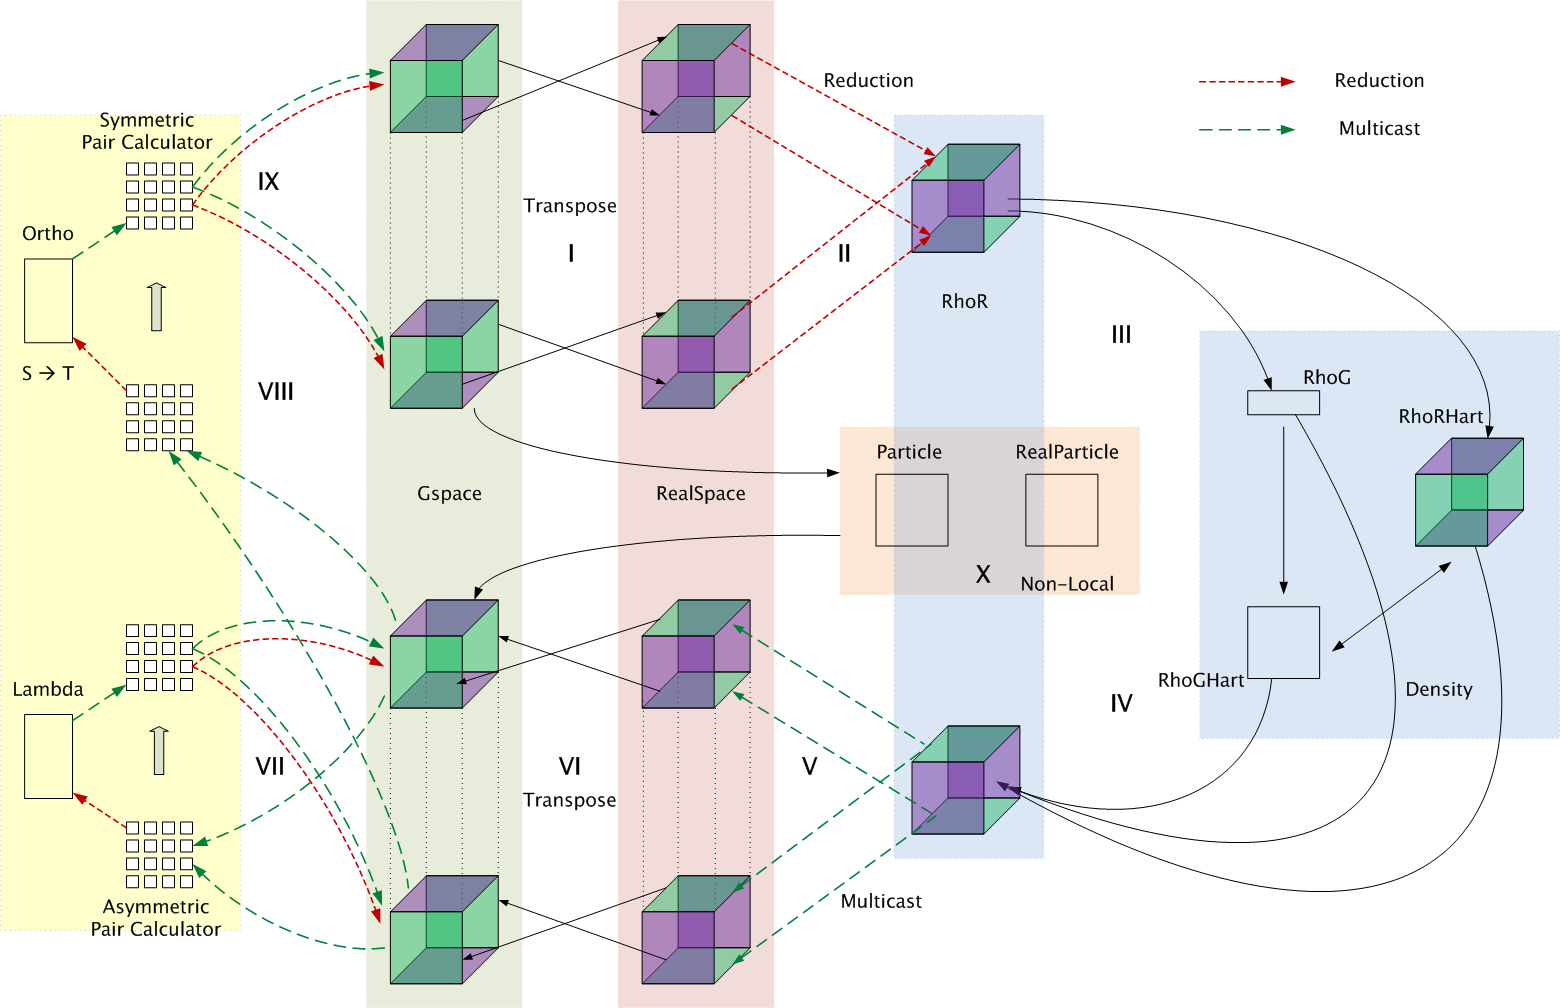
\includegraphics[width=5in]{OpenAtomDiagram} 
\caption{Flow of control in \leancp{}} 
\label{fig:leancp} 
\end{figure} 

\begin{itemize}
\item{\bf Phase I:} In this phase, the real-space representation of the 
electronic states is obtained from the g-space representation through a 
transpose based 3-dimensional Fast Fourier Transform (FFT). 

\item{\bf Phase II:} Electron density in real-space is obtained via reductions
from the real-space state representation.

\item{\bf Phase III:} Fourier components of the density in g-space are created
from the corresponding copy in real-space through a 3D FFT.

\item{\bf Phase IV:} Once we have the g-space copy, it is used to compute the
``Hartree and external energies" via multiple 3D FFTs which can be performed
independently.

\item{\bf Phase V:} The energies computed in the previous phase are reduced
across all processors and send to the corresponding planes of the different 
states through multicasts. This is exactly reverse of the procedure used to 
obtain the density in phase II.

\item{\bf Phase VI:} In this phase, the forces are obtained in g-space from
real-space via a 3D FFT.

\item{\bf Phase VII:} For functional minimization, force regularization is done
in this phase by computing the overlap matrix Lambda ($\Lambda$) and applying 
it. This involves several multicasts and reductions.

\item{\bf Phase VIII:} This phase is similar to Phase VII and involves
computation of the overlap matrix Psi ($\Psi$) and its inverse square root 
(referred to as the S $\rightarrow$ T process) to obtain ``reorthogonalized" 
states. This phase is called orthonormalization.

\item{\bf Phase IX:} The inverse square matrix from the previous phase is
used in a ``backward path" to compute the necessary modification to the
input data. This again involves multicasts and reductions to obtain the input
for phase I of the next iteration.

\item{\bf Phase X:} Since Phase V is a bottleneck, this phase is interleaved 
with it to perform the non-local energy computation. It involves computation of
the kinetic energy of the electrons and computation of the non-local 
interaction between electrons and the atoms using the EES method~\cite{EESNL}.
\end{itemize}

For a detailed description of this algorithm please refer to~\cite{LeanCPIBM07}.
We will now proceed to understand the communication involved in these phases
through a description of the various chare arrays involved and dependencies
among them.

%%%%%%%%%%%%%%%%%%%%%%%%%%%%%%%%%%%%%%%%%%%%%%%%%%%%%%%%%%%%%%%%%%%%%%%%%%%%%%
\section{Communication in \leancp{}}
The ten phases described in the previous section are parallelized by
decomposing the physical system into 15 chare arrays of different dimensions 
(ranging between one and four). A description of these objects and communication
between them follows:

\begin{enumerate}
\item {\bf GSpace and RealSpace:} These represent the g-space and real-space 
representations of the electronic states. They are 2-dimensional arrays 
with states in one dimension and planes in the other. They are represented by
$G(s, p)\ [n_s \times N_g]$ and $R(s, p)\ [n_s \times N]$ respectively. GSpace
and RealSpace interact through transpose operations in Phase I and hence all 
planes of one state of GSpace interact with all planes of the same state of 
RealSpace. RealSpace also interacts with RhoR through reductions in Phase II.

\item {\bf RhoG and RhoR:} They are the g-space and real-space representations of
electron density and are 1-dimensional (1D) and 2-dimensional (2D) arrays
respectively. They are represented as $G_{\rho}(p)\ [N_{g \rho}]$ and 
$R_{\rho}(p, p')\ [(N / N_y) \times N_y]$. RhoG is obtained from RhoR in Phase
III through two transposes.

\item {\bf RhoGHart and RhoRHart:} RhoR and RhoG are used to compute their 
Hartree and exchange energy counterparts through several 3D FFTs (in Phase IV). 
This involves transposes and point-to-point communication. RhoGHart and RhoRHart
are 2D and 3D arrays represented by $G_{HE}(p, a)\ [N_{gHE} \times 
n_{atom-type}]$ and $R_{HE}(p, p',$ $a)\ [(1.4N / N_y) \times N_y \times 
n_{atom-type}]$.

\item {\bf Particle and RealParticle:} These two 2D arrays are the g-space and
real-space representations of the non-local work and denoted as $G_{nl}(s, p)\
[n_s \times N_g]$ and $R_{nl}(s, p)\ [n_s \times 0.7N]$. Phase X for the
non-local computation can be overlapped with Phases II-VI and involves
communication for two 3D FFTs.

\item {\bf Ortho and CLA\_Matrix:} The 2D ortho array, $O(s, s')$ does the 
post-processing of the overlap matrices to obtain the T-matrix from the 
S-matrix. There are three 2D CLA\_Matrix instances used in each of the steps of
the inverse square method (for matrix multiplications) used during 
orthonormalization. In the process, these arrays 
communicate with the paircalculator chare arrays mentioned next. 

\item {\bf PairCalculators:} These 4-dimensional (4D) arrays are used in the 
force regularization and orthonormalization phases (VII and VIII). They 
communicate with the GSpace, CLA\_Matrix and Ortho arrays through multicasts and
reductions. They are represented as $P_c(s, s', p, p')$ of dimensions $n_s 
\times n_s \times N_g \times N_{g}'$. A particular state of the GSpace array 
interacts with all elements of the paircalculator array which have this state in
one of its first two dimensions.

\item {\bf Structure Factor:} This is a 3D array used when we do not use the 
EES method for the non-local computation.
\end{enumerate}

\bibliographystyle{unsrt}
\bibliography{other}

\end{document}
